\section{Dependency Plan}

\begin{figure}[H]
	\centering
	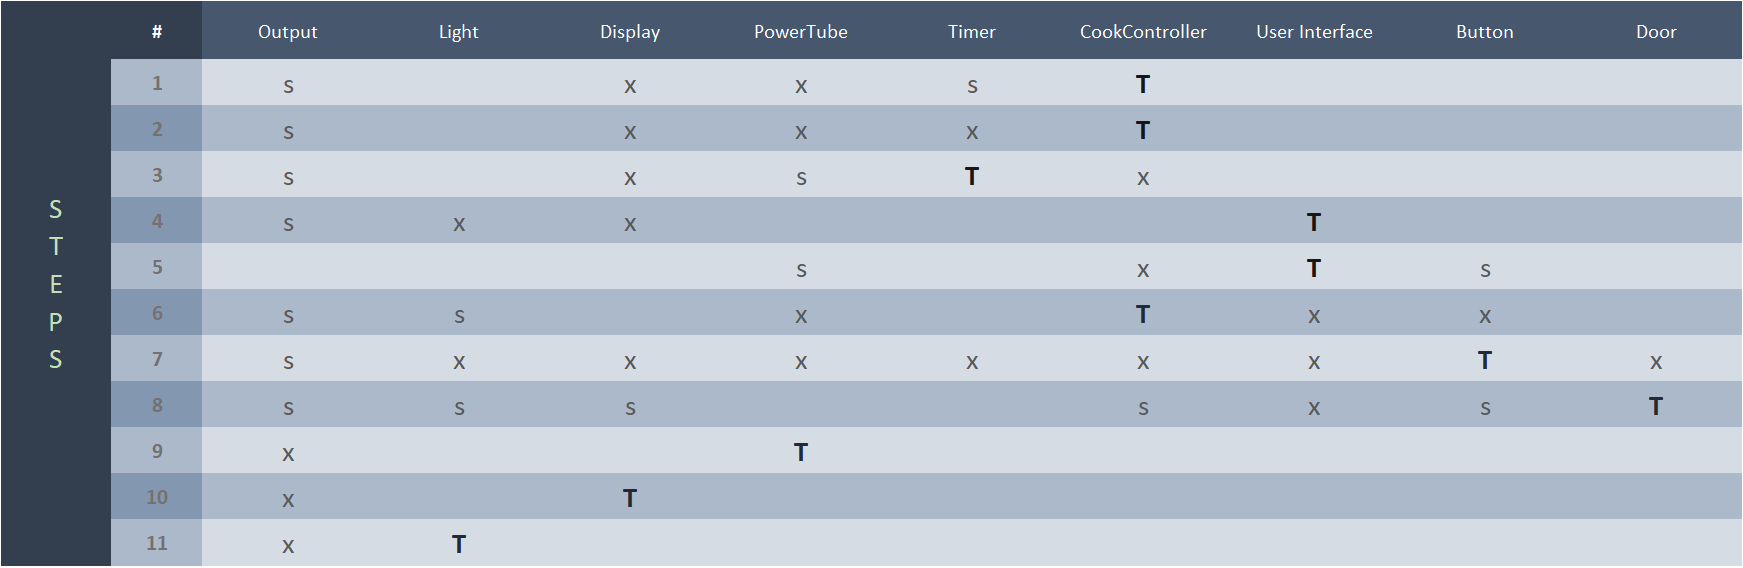
\includegraphics[width=1\linewidth]{../Diagrams/IntegrationPlan}
	\caption[Integration Plan]{}
	\label{fig:integrationplan}
\end{figure}

\subsection{Valg for Integrations plan}
begrundelse hvorfor bedste patterns (første udkast bottom up, top-down)
hovedpointen i bottom up metoden er at man kan integrations teste systemet ved start af de komponenter med færrest afhængigheder. dvs komponenter med færrest afhængigheder testes først. Når disse komponenter er blevet testet og godkendt så kan man rykker videre til de næste komponenter indtil hele systemet er blevet testet. \medskip
Fordelen ved bottom op er at vi kan hurtigt går i gang med at integerer en smule af systemet. der kan integeres parallelt hvis projektet er stort. I andre ord, så kan der være flere udvikler der arbejder samtidigt på systemets test. Da de ikke er afhængig af de andre udviklers integrationstest. \medskip
Set ud fra vores afhængighedstræ er der en del komponenter der afhænger af andre komponenter i afhængigheds træet. derfor tænker vi at det vil være oplagt at anvende bottom op metoden.

